% siminos/talks/GTmath12/sectSlice.tex      pdflatex sectSlice
% $Author: burak $
% $Date: 2014-04-11 17:09:12 -0400 (Fri, 11 Apr 2014) $

% remember to always update
%	dasbuch/WWW/overheads/continuous/continuous.pdf

% Predrag GT math colloquium                2012.03.26
% derived from
% talks/predrag/continuous/continuous.tex   2011.09.09
% Predrag beamer format                     2011.06.17
% Predrag                                   2011.04.12
% derived from
% siminos/talks/Dresden10/symmReduc.tex 	2010.06.29
% Predrag Eckmann's haeberli slide style    2005.05.03
%    ChaosBook/version 11 slides
%	 from ChaosBook continuous.tex

% might want to use text from
%    predrag/lectures/Goth11/Cphg11abstr.txt
%    predrag/lectures/maribor/11/abscvitancourse.tex

\input ../../inputs/layoutBeamer
\input ../../inputs/def % no edits, always from dasbuch/book/inputs
\input ../../inputs/defsBeamer
                          \date{\textcolor{yellow}{\scriptsize
 16 March 2012
                          }}

\title{{\Huge got symmetry?}
       \\
       {here is how you slice it}}
%\author{Predrag Cvitanovi\'c}
\author[Cvitanovi\'c]
{
  \textcolor{green!50!black}{
  {Predrag~Cvitanovi\'c}
  }
}
\institute
{
%  \inst{1}%
CDSNS Colloquium \\
School of Mathematics, Georgia Tech
}

\begin{document}

\begin{frame}
  \titlepage
\end{frame}

%\begin{frame}{Outline}
%  \tableofcontents
%\end{frame}

\section[dynamical systems]{dynamical systems}

\subsection[dynamical systems]{dynamical systems}

\begin{frame}{dynamical description of turbulent flows}
%	from {../chapter/dynsysII}

\begin{block}{\statesp}
a manifold $\pS \in \reals^{d}$ :
$d$ numbers determine the state of the system
\end{block}

\bigskip

\begin{block}{representative point }
$\ssp(t) \in \pS$
\\
a state of physical system at instant in time
\end{block}
\end{frame}

\begin{frame}{today's experiments}
\begin{block}{example of a representative point }
$\ssp(t) \in \pS$, $d= \infty$ \\
a state of turbulent pipe flow at instant in time
\end{block}

\bigskip

%%%%%%%%%%%%%%%%%%%%%%%%%%%%%%%%%%%%%%%%%%%%%%%%%%%%%%%%%%%%%%%%%%
%\hfill
%\begin{minipage}[c]{0.35\textwidth}
Stereoscopic Particle Image Velocimetry $\to$
3-$d$ velocity field over the entire pipe%
\footnote{
%"Stereoscopic PIV on transition in pipe flow",
Casimir W.H. van Doorne
(PhD thesis, Delft  2004)
%; 	{\tt www.ahd.tudelft.nl}
}

\bigskip

\begin{center}
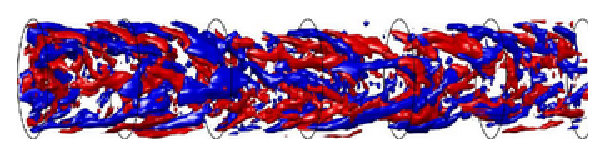
\includegraphics[width=0.90\textwidth]{vDoorne4}
\end{center}
\end{frame}

\begin{frame}{}
\begin{block}{deterministic dynamics}
map $\timeflow(\xInit)$ =
representative point time $t$ later
\end{block}

\begin{block}{evolution}
\begin{center}
\includegraphics[width=0.40\textwidth]{f_flow}
\end{center}
$\timeflow$ maps a region $\pS_i$ of
the {\statesp} into the region $\flow{t}{\pS_i}$.
\end{block}
\end{frame}

\begin{frame}{have : chart over 61,506 dimensional \statesp\ of turbulent flow}
\begin{center}
\includegraphics[width=0.80\textwidth]{statespace_123}
\end{center}
\eqva\ of turbulent plane Couette flow,
their unstable manifolds, and a turbulent video mapped out as one happy family

\bigskip

\hfill   {\small
          for movies, please click through
            \textcolor{blue}{\href{http://ChaosBook.org/tutorials}
             {ChaosBook.org/tutorials}}
          }
\end{frame}

%%%%%%%%%%%%%%%%%%%%%%%%%%%%%%%%%%%%%%%%%%%%%%%%%%%%%%%%%%%%%%%%%%%%%%%%%%%%
\section[Das Problem]{the problem with symmetry}


\begin{frame}{}
today's talk's focus:
\begin{block}{}
{\Huge
nature loves symmetry
}
\end{block}
\end{frame}

\begin{frame}{symmetry of a dynamical system}
\begin{block}{a group $\Group$ is a {symmetry} of the dynamics if}
for every solution $f(\ssp) \in \pS$ and  $\LieEl \in \Group$,
$\LieEl f(\ssp)$ is also a solution
\end{block}
\end{frame}


\begin{frame}{example: $\SOn{2}_z\times \On{2}_\theta$ symmetry of pipe flow}
            \begin{block}{}
 %% A27*-pipeSymms.* - read dasbuch/book/FigSrc/inkscape/00ReadMe.txt
 \begin{center}
  \setlength{\unitlength}{0.35\textwidth}
  %% \unitlength = units used in the Picture Environment
(a)
  \begin{picture}(1,0.52454249)%
    \put(0,0){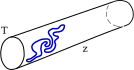
\includegraphics[width=\unitlength]{A27a-pipeSymms}}%
    \put(0.61583231,0.13683004){\color[rgb]{0,0,0}\makebox(0,0)[lb]{\smash{$z$}}}%
    \put(0.00611823,0.27217453){\color[rgb]{0,0,0}\makebox(0,0)[lb]{\smash{$\theta$}}}%
  \end{picture}%
(b)
  \begin{picture}(1,0.52454249)%
    \put(0,0){\includegraphics[width=\unitlength]{A27b-pipeSymms}}%
    \put(0.61583231,0.13683004){\color[rgb]{0,0,0}\makebox(0,0)[lb]{\smash{$z$}}}%
    \put(0.00611823,0.27217453){\color[rgb]{0,0,0}\makebox(0,0)[lb]{\smash{$\theta$}}}%
  \end{picture}%
\\
(c)
  \begin{picture}(1,0.52454249)%
    \put(0,0){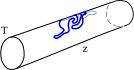
\includegraphics[width=\unitlength]{A27c-pipeSymms}}%
    \put(0.61583231,0.13683004){\color[rgb]{0,0,0}\makebox(0,0)[lb]{\smash{$z$}}}%
    \put(0.00611823,0.27217453){\color[rgb]{0,0,0}\makebox(0,0)[lb]{\smash{$\theta$}}}%
  \end{picture}%
(d)
  \begin{picture}(1,0.52454249)%
    \put(0,0){\includegraphics[width=\unitlength]{A27d-pipeSymms}}%
    \put(0.61583231,0.13683004){\color[rgb]{0,0,0}\makebox(0,0)[lb]{\smash{$z$}}}%
    \put(0.00611823,0.27217453){\color[rgb]{0,0,0}\makebox(0,0)[lb]{\smash{$\theta$}}}%
  \end{picture}%
 \end{center}
a solution, shifted by a stream-wise translation, azimuthal rotation
$g_p$ is also a solution
			\end{block}
%	\end{columns}
% \caption{\label{fig:A27-pipeSymms}
			\begin{exampleblock}{}
\begin{itemize}
  \item[b)]  stream-wise
  \item[c)]  stream-wise, azimuthal
  \item[d)]  azimuthal flip
\end{itemize}
			\end{exampleblock}
\end{frame}


\subsection[{\cLf} example]{prelude: {\cLf} example}

\begin{frame}{\Large Das Problem}
\begin{block}{}
    {\large
% physicists
mathematicians like symmetry more than Nature
    }

\bigskip

\hfill
Rich Kerswell
\end{block}
\end{frame}

\begin{frame}{turbulence in pipe flows}
pipe flows : amazing data! amazing numerics!
\begin{center}
  \includegraphics[width=1.0\textwidth,clip=true]
                    {pipeSects}
\end{center}

\bigskip
Nature, she don't care :
turbulence breaks all symmetries
\end{frame}

\begin{frame}{\Large Die Faulheit}
\begin{block}{drifting is energetically cheap}
flows are lazy, rather than doing work, solutions drift along non-shape-changing
symmetry directions
\end{block}
\end{frame}



\begin{frame}{\Large Das Problem}
% \begin{frame}{from {\cLf} $5D$ attractor $\to$ unimodal map}
	\begin{columns}[t]
	\column{.6\textwidth}
			\begin{exampleblock}{{\cLe}}
\scriptsize		
\[
		\left[
					\begin{array}{c}
				\dot{x}_1 \\ \dot{x}_2 \\ \dot{y}_1 \\ \dot{y}_2 \\ \dot{z}
				\end{array}
		\right]
=
		\left[
					\begin{array}{c}
				 -\sigma x_1 + \sigma y_1 \\
				-\sigma x_2 + \sigma y_2 \\
                (\RerCLor-z) x_1 - \ImrCLor x_2 -y_1-e y_2 \\
                \ImrCLor x_1 + (\RerCLor-z) x_2 + e y_1- y_2 \\
				-b z + x_1 y_1 + x_2 y_2
				\end{array}
		\right]
\]
$\RerCLor=28, \ImrCLor=0, b=8/3, \sigma=10, e= 1/10$
			\end{exampleblock}
            \begin{block}{}
  \begin{itemize}
  \item A typical $\{x_1,x_2,z\}$ trajectory
  \item superimposed:
  a trajectory  whose initial
  point is close to the \reqv\ $Q_{1}$
  \end{itemize}
            \end{block}
	\column{.40\textwidth}
 		\begin{exampleblock}{attractor}
        \includegraphics[width=\textwidth,clip=true]
                        {CLEx1x2z} %CLEx1x2zRelEqu}
		\end{exampleblock}
	\end{columns}
\end{frame}

\begin{frame}{} %{\statesp\ portrait of \cLf\ solutions}
\begin{block}{continuous symmetry induces drifts}
\begin{center}
  \includegraphics[width=0.35\textwidth,clip=true] %,height=0.5\textheight
  {CLEchaotic}
  \includegraphics[width=0.35\textwidth,clip=true]
  {CLEcompact}
\end{center}
\end{block}
\begin{itemize}
  \item generic chaotic trajectory (blue)
  \item $E_0$ \eqv  %\EQV{0}
  \item $E_0$ unstable manifold - a cone of such (green)
  \item $Q_1$ \reqv\ (red)
  \item $Q_1$ unstable manifold, one for each point on $Q_1$ (brown)
  \item \rpo\ \cycle{01} (purple)
\end{itemize}
\end{frame}

\begin{frame}{
         \only<1>{
Das Durcheinander
         }
         \only<2>{
\Large Die L\"osung
        }
            }
% \begin{frame}{from {\cLf} $5D$ attractor $\to$ unimodal map}
	\begin{columns}[t]
	\column{.6\textwidth}
			\begin{block}{what to do?}
it's a mess
			\end{block}
			\begin{block}{the goal}
 reduce this messy strange attractor
to something simple
			\end{block}
	\column{.40\textwidth}
         \only<1>{
		\begin{exampleblock}{attractor}
        \includegraphics[width=\textwidth,clip=true]
                        {CLEx1x2z} %CLEx1x2zRelEqu}
		\end{exampleblock}
                }
         \only<2>{
		\begin{exampleblock}{symmetry \reducedsp}
  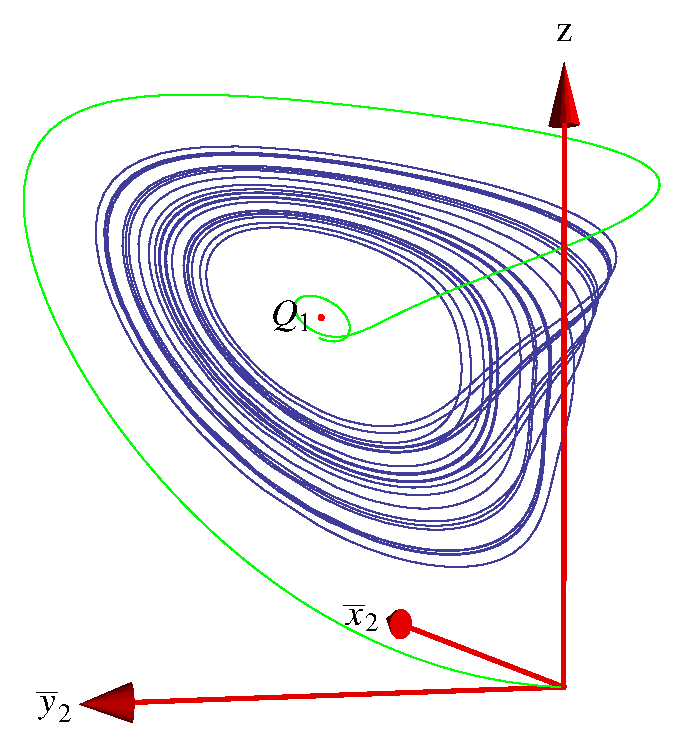
\includegraphics[width=\textwidth,clip=true]
  {CLEinvXYZ} %CLEip1}
		\end{exampleblock}
        \hfill  \textcolor{red}{amazing!}
                }
	\end{columns}
\end{frame}

\begin{frame}{\Large Das Gebot}
\begin{block}{}
    {\large
what I teach you now you must do
    }
\end{block}
\end{frame}

\section[relativity for cyclists]{relativity for cyclists}

\subsection[in/equivariance]{}

\begin{frame}{symmetries of dynamics}
  \begin{columns}
  \column{0.45\textwidth}
\begin{block}{time vs. shifts}
%\label{fig:tangents}
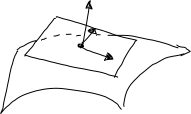
\includegraphics[width=0.90\textwidth]{A27groupTan}
\end{block}
  \column{0.55\textwidth}
$\vel(\ssp)$ : tangent along the time flow

\bigskip

$\groupTan^{(1)}(\ssp)$, $\groupTan^{(2)}(\ssp)$ : two group tangents
along infinitesimal symmetry shifts
	\end{columns}

\bigskip

\begin{block}{a flow $\dot{\ssp}= \vel(\ssp)$ is $\Group$-equivariant if}
\[
\vel(\ssp)=\LieEl^{-1} \, \vel(\LieEl \, \ssp)
\,,\qquad \mbox{for all } \LieEl \in {\Group}
\,.
\] %ee{eq:FiniteRot}

\end{block}

\bigskip

\hfill equations of motion of the same form in all frames
\end{frame}

\begin{frame}{example: \SOn{2} invariance}
			\begin{exampleblock}{{\cLe}}
\scriptsize		
\[
		\left[
					\begin{array}{c}
				\dot{x}_1 \\ \dot{x}_2 \\ \dot{y}_1 \\ \dot{y}_2 \\ \dot{z}
				\end{array}
		\right]
=
		\left[
					\begin{array}{c}
				 -\sigma x_1 + \sigma y_1 \\
				-\sigma x_2 + \sigma y_2 \\
                (\RerCLor-z) x_1 - \ImrCLor x_2 -y_1-e y_2 \\
                \ImrCLor x_1 + (\RerCLor-z) x_2 + e y_1- y_2 \\
				-b z + x_1 y_1 + x_2 y_2
				\end{array}
		\right]
\]
			\end{exampleblock}

\begin{block}{}
invariant under a \SOn{2} rotation by finite angle
\gSpace:
\scriptsize		
\[
\LieEl(\gSpace) \,=\,  \left(\barr{ccccc}
  \cos \gSpace  & \sin \gSpace  & 0 & 0 & 0 \\
 -\sin \gSpace  & \cos \gSpace  & 0 & 0 & 0 \\
 0 & 0 &  \cos \gSpace & \sin \gSpace   & 0 \\
 0 & 0 & -\sin \gSpace & \cos \gSpace   & 0 \\
 0 & 0 & 0             & 0              & 1
    \earr\right)
\] %{CLfRots}
\end{block}
%\begin{block}{\statesp\ decomposition}
%\begin{enumerate}
%  \item $m=0$ \SOn{2}-invariant subspace: $z$-axis
%  \item $m=1$ subspace with multiplicity 2
%\end{enumerate}
%\end{block}
\end{frame}

\begin{frame}{trajectories, orbits}
%  \caption{\label{fig:A27wurst}
	\begin{columns}[t]
	\column{.32\textwidth}
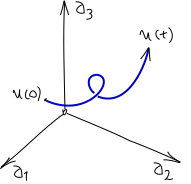
\includegraphics[width=0.95\textwidth]{A27traj}

trajectory $\ssp(\zeit)$
	\column{.32\textwidth}
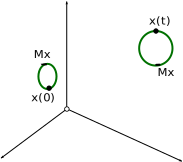
\includegraphics[width=0.95\textwidth]{A27gOrbit}

group orbit $\LieEl\,\ssp(0)$
	\column{.32\textwidth}
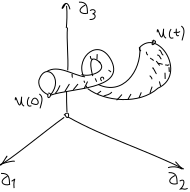
\includegraphics[width=0.95\textwidth]{A27wurst}

wurst $\LieEl\,\ssp(\zeit)$
	\end{columns}
\end{frame}

\begin{frame}{stratification by group orbits}
  \begin{columns}
  \column{0.5\textwidth}
\begin{block}{group orbits}
% 2011-08-23 Predrag: previously BeThTraj.pdf from
% dasbuch/book/FigSrc/inkscape/BeThTraj.svg
%  2011-09-09 Predrag: updated continuous.tex overheads
%  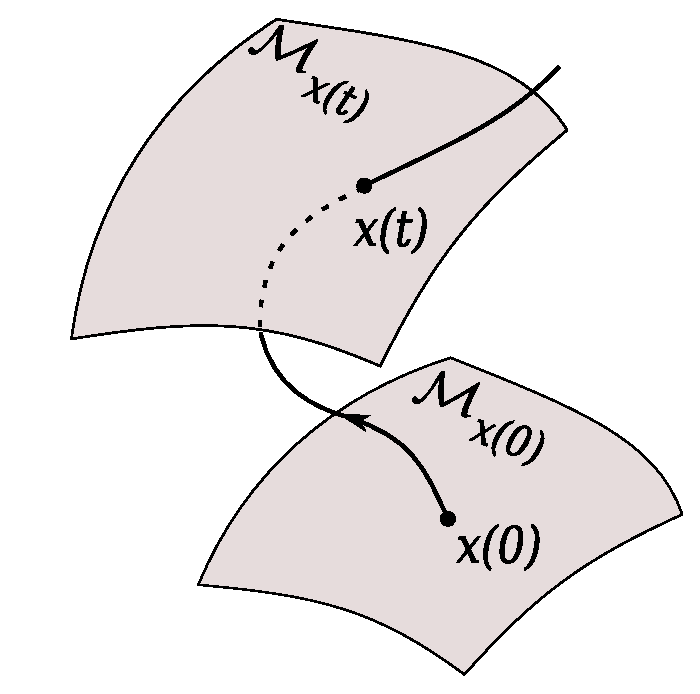
\includegraphics[width=1.00\textwidth,clip=true]{BeThTraj}
 \begin{center}
  \setlength{\unitlength}{1.00\textwidth}
  %% \unitlength = units used in the Picture Environment
  \begin{picture}(1,1.07471658)%
    \put(0,0){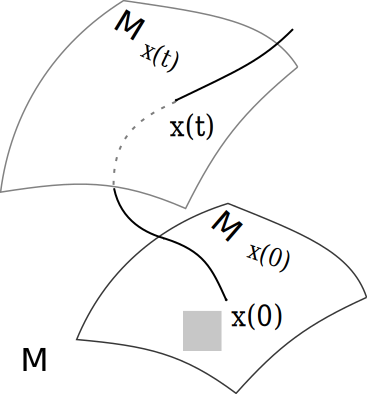
\includegraphics[width=\unitlength]{BeThTrajTeX}}%
    \put(0.28879298,1.02196543){\color[rgb]{0,0,0}\rotatebox{-22.37140782}{\makebox(0,0)[lb]{\smash{$\pS_{\ssp(\tau)}$}}}}%
    \put(0.55566402,0.45078735){\color[rgb]{0,0,0}\rotatebox{-16.6673442}{\makebox(0,0)[lb]{\smash{$\pS_{\ssp(0)}$}}}}%
    \put(0.63028127,0.18433597){\color[rgb]{0,0,0}\rotatebox{0.03136739}{\makebox(0,0)[lb]{\smash{$\ssp(0)$}}}}%
    \put(0.46253394,0.70182304){\color[rgb]{0,0,0}\rotatebox{0.03136739}{\makebox(0,0)[lb]{\smash{$\ssp(\tau)$}}}}%
    \put(0.03852492,0.09250899){\color[rgb]{0,0,0}\rotatebox{0.11031334}{\makebox(0,0)[lb]{\smash{$\pS$}}}}%
  \end{picture}%
 \end{center}
\end{block}
  \column{0.5\textwidth}
		\only<1>{
\noindent
\emph{group orbit} $\pS_\ssp $ of $\ssp$ is the set of all group
actions
\[
\pS_\ssp = \{\LieEl\,\ssp \mid \LieEl \in {\Group}\}
\]
        }
		\only<2>{
%\noindent
%group orbit $\pS_{\ssp(0)}$ of \statesp\ point
% $\ssp(0)$, and the group orbit $\pS_{\ssp(t)}$
%reached by the trajectory $\ssp(t)$ time $t$ later.
%        }
%		\only<3>{
\noindent
any point on the manifold $\pS_{\ssp(t)}$ is
equivalent to any other
        }
		\only<3>{
\noindent
action of a symmetry group
stratifies the \statesp\ into a union of group
orbits

\medskip

each group orbit an equivalence class
        }
\end{columns}
\end{frame}

\section{symmetry reduction}

\begin{frame}{}
\begin{block}{the goal}
replace each group orbit by a unique
point in a lower-dimensional

\bigskip

\hfill
\textcolor{red}{\Large symmetry \reducedsp\ $\pS/\Group$}
\end{block}
\end{frame}

\begin{frame}{symmetry reduction}
  \begin{columns}
  \column{0.5\textwidth}
\begin{block}{full \statesp}
 \begin{center}
  \setlength{\unitlength}{1.00\textwidth}
  %% \unitlength = units used in the Picture Environment
  \begin{picture}(1,1.07315413)%
    \put(0,0){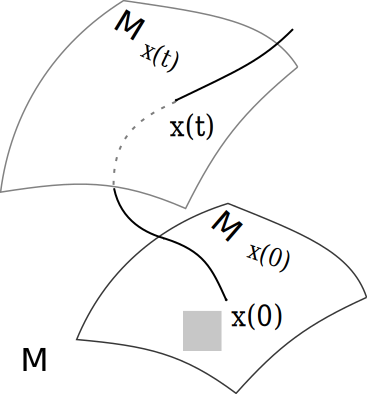
\includegraphics[width=\unitlength]{BeThTrajTeX}}%
    \put(0.30362031,0.99939308){\color[rgb]{0,0,0}\rotatebox{-31.32889204}{\makebox(0,0)[lb]{\smash{$\pS_{\ssp(\tau)}$}}}}%
    \put(0.5686188,0.45975596){\color[rgb]{0,0,0}\rotatebox{-40.8073288}{\makebox(0,0)[lb]{\smash{$\pS_{\ssp(0)}$}}}}%
    \put(0.63028127,0.18433598){\color[rgb]{0,0,0}\rotatebox{0.03136739}{\makebox(0,0)[lb]{\smash{$\ssp(0)$}}}}%
    \put(0.46253394,0.70182305){\color[rgb]{0,0,0}\rotatebox{0.03136739}{\makebox(0,0)[lb]{\smash{$\ssp(\tau)$}}}}%
  \end{picture}%
 \end{center}
\end{block}
  \column{0.5\textwidth}
\begin{block}{\reducedsp}
 \begin{center}
  \setlength{\unitlength}{1.00\textwidth}
  %% \unitlength = units used in the Picture Environment
  \begin{picture}(1,1.07315413)%
    \put(0,0){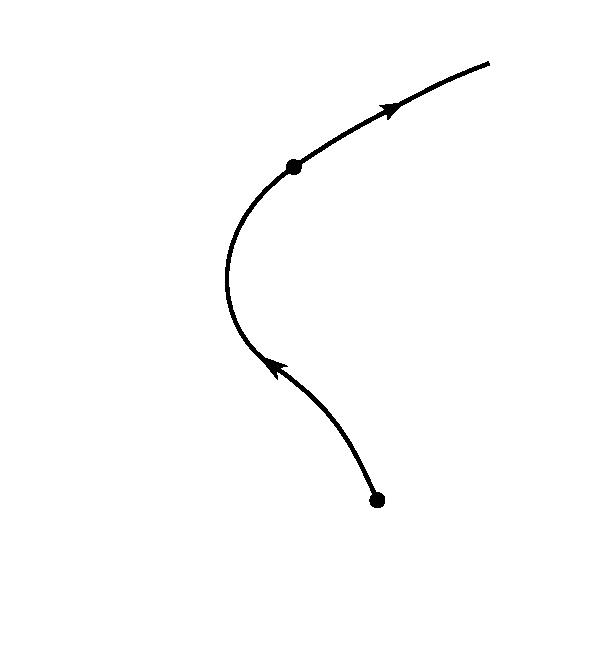
\includegraphics[width=\unitlength]{BeThRedTeX}}%
    \put(0.19912369,0.17144733){\color[rgb]{0,0,0}\rotatebox{0.11031334}{\makebox(0,0)[lb]{\smash{$\pSRed$}}}}%
    \put(0.63028127,0.18433598){\color[rgb]{0,0,0}\rotatebox{0.03136739}{\makebox(0,0)[lb]{\smash{$\sspRed(0)$}}}}%
    \put(0.46253394,0.70182305){\color[rgb]{0,0,0}\rotatebox{0.03136739}{\makebox(0,0)[lb]{\smash{$\sspRed(\tau)$}}}}%
  \end{picture}%
 \end{center}
\end{block}
\end{columns}
\end{frame}

\begin{frame}{moving frame}
  \begin{columns}
  \column{0.45\textwidth}
\begin{block}{}
%\label{fig:A27movFrame}
  \setlength{\unitlength}{1.00\textwidth}
  \begin{picture}(1,0.95956879)%
    \put(0,0){\includegraphics[width=\unitlength]{A27movFrame1}}%
    \put(0.23452859,0.20577397){\color[rgb]{0,0,0}\rotatebox{13.70564637}{\makebox(0,0)[lb]{\smash{$\ssp(0)$}}}}%
    \put(0.33101524,0.7744554){\color[rgb]{0,0,0}\rotatebox{25.42186498}{\makebox(0,0)[lb]{\smash{$\ssp(\zeit)$}}}}%
    \put(0.8633058,0.79722561){\color[rgb]{0,0,0}\rotatebox{-35.54161781}{\makebox(0,0)[lb]{\smash{$\sspRed(\zeit)$}}}}%
    \put(0.61945216,0.80401789){\color[rgb]{0,0,0}\makebox(0,0)[lb]{\smash{$\LieEl(\zeit)$}}}%
  \end{picture}%
\end{block}
  \column{0.55\textwidth}
Cartan : can move wherever
	\end{columns}

\bigskip

free to redefine the flow to any time-dependent frame moving
along symmetry directions
\end{frame}


\begin{frame}{how relativists do it : connections or `gauge fixing'}
2-continuous parameter symmetry :

each \statesp\ point $\ssp$ owns 3 tangent vectors

\bigskip

  \begin{columns}
  \column{0.45\textwidth}
\begin{block}{local tangent space}
%\label{fig:tangents}
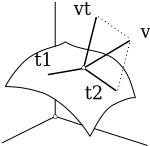
\includegraphics[width=0.80\textwidth]{A28tangents}
\end{block}
  \column{0.55\textwidth}

$\vel(\ssp)$ along the time flow

\bigskip

$\groupTan^{(1)}(\ssp)$, $\groupTan^{(2)}(\ssp)$
along infinitesimal symmetry shifts
	\end{columns}

\begin{block}{Kim Jong Il gauge}
follow flow $\velRed(\ssp)$  normal to group tangent directions
\end{block}
\end{frame}

\begin{frame}{method of ``connections''}
%\label{fig:A28extremum}
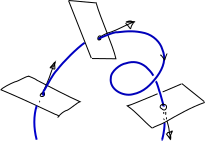
\includegraphics[width=0.60\textwidth]{A28mConnect}

\bigskip

never stray along the group directions, always move orthogonally to
the group orbit

\bigskip

North Korean gauge :

slacking along non-shape-changing directions is forbidden
\end{frame}


\begin{frame}{sophisticates do it : Faddeev-Popov gauge fixing}
\begin{block}{the equivalence principle}
integrate over classes of gauge equivalent fields
\\
instead of all fields $A_\mu^a$
\end{block}

the representative in the class of equivalent fields is
fixed by a gauge condition,
\[
    \partial_{\mu} A_{\mu}^{a} = 0
    \,,
\]
a plane intersected by the gauge orbits
\[
    A_{\mu} = A_{\mu}^{a}t_{a} \to A_{\mu}^{\Omega}
            = \Omega A_{\mu} \Omega^{-1} + \partial_{\mu} \Omega \Omega^{-1}
\]
\begin{itemize}
  \item abelian orbits intersect the plane at the same angle
  \item non-abelian intersection angle depends on the field
\end{itemize}
\end{frame}

\begin{frame}{\Large Zutiefst Nutzlos}
\begin{block}{}
    {\large
elegant, deep and useless : no symmetry reduction
    }
\end{block}
\end{frame}


\section[slice n' dice]{slice n' dice}

\begin{frame}{relativity for cyclists}
\begin{block}{\mslices}

\bigskip
cut group orbits by a hypersurface
\textcolor{red}{(not a Poincar\'e section)}, each group orbit of
symmetry-equivalent points represented by the single point
\end{block}
\bigskip
\textcolor{blue}{\Large cut how?}
\end{frame}


\begin{frame}{inspiration: pattern recognition}
you are observing turbulence in a pipe flow, or your defibrillator has a
mesh of sensors measuring electrical currents that cross your heart, and

\medskip

you have a precomputed pattern, and are sifting through the data set of
observed patterns for something like it

\medskip

here you see a pattern, and there you see a pattern that seems much like
the first one

\bigskip

\bigskip

\textcolor{red}{\Large how `much like the first one?'}
\end{frame}

\begin{frame}{moving frame}
  \begin{columns}
  \column{0.45\textwidth}
\begin{block}{}
%\label{fig:A27movFrame}
  \setlength{\unitlength}{1.00\textwidth}
  \begin{picture}(1,0.95956879)%
    \put(0,0){\includegraphics[width=\unitlength]{A27movFrame1}}%
    \put(0.23452859,0.20577397){\color[rgb]{0,0,0}\rotatebox{13.70564637}{\makebox(0,0)[lb]{\smash{$\ssp(0)$}}}}%
    \put(0.33101524,0.7744554){\color[rgb]{0,0,0}\rotatebox{25.42186498}{\makebox(0,0)[lb]{\smash{$\ssp(\zeit)$}}}}%
    \put(0.8633058,0.79722561){\color[rgb]{0,0,0}\rotatebox{-35.54161781}{\makebox(0,0)[lb]{\smash{$\sspRed(\zeit)$}}}}%
    \put(0.61945216,0.80401789){\color[rgb]{0,0,0}\makebox(0,0)[lb]{\smash{$\LieEl(\zeit)$}}}%
  \end{picture}%
\end{block}
  \column{0.55\textwidth}
move until distance minimized
	\end{columns}
\end{frame}


\begin{frame}{}
take the first pattern
\begin{block}{`template' or `reference state'}
\hfill  a point {\slicep} in the \statesp\  \pS
\end{block}

and use the symmetries of the flow to
\begin{block}{slide and rotate the `{\template}'}
\hfill  act with elements of the symmetry group \Group\ on
$\slicep \to \LieEl(\gSpace)\,\slicep$
\end{block}
 until it overlies the second pattern (a point $\ssp$ in
the \statesp)
\begin{block}{distance between the two patterns}
\[ %beq
|\ssp - \LieEl(\gSpace)\,\slicep|
    = |\sspRed - \slicep|
%\label{minDistance}
\] %eeq
\end{block}
is minimized
\end{frame}

\begin{frame}{idea: the closest match}
  \begin{columns}
  \column{0.60\textwidth}
\begin{block}{} %group orbits}
\begin{center}
  \includegraphics[width=1.00\textwidth,clip=true]
  {sliceLie}
\end{center}
\end{block}
  \column{0.40\textwidth}
template: Sophus Lie

\bigskip
(1) rotate bearded guy $\ssp$
\\
\textcolor{blue}{traces out the group orbit $\pS_\ssp$}

\bigskip
(2) replace the group orbit by the closest match $\sspRed$
to the template pattern $\slicep$

\bigskip
the closest matches $\sspRed$ lie in the $(d\!-\!N)$ symmetry \reducedsp\
$\pSRed$
\end{columns}
\end{frame}

\begin{frame}{distance}
assume that \Group\
is a subgroup of the group of orthogonal transformations
$\On{d}$, and measure
distance $|\ssp|^2=\braket{\ssp}{\ssp}$ in terms of the Euclidean inner
product

\bigskip
numerical fluids:  PDE discretization independent L2 distance is
\begin{block}{energy norm}
\[
  \Norm{\bu-\bv}^2  = \braket{\bu-\bv}{\bu-\bv}  = \frac{1}{V}
                \int_\bCell \! d \bx \;
                       (\bu-\bv) \cdot (\bu-\bv)
%\label{innerproduct}
\]
\end{block}

\bigskip
experimental fluid:
\begin{block}{image discretization independent distance}
 is Hamming distance, or ???
\end{block}
\end{frame}

\subsection{\mslices}

\begin{frame}{idea: the closest match}
%\label{fig:A28extremum}
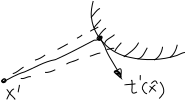
\includegraphics[width=0.60\textwidth]{A28extremum}

extremal condition for nearest distance
\end{frame}

\begin{frame}{}
\begin{block}{minimal distance}
is a solution to the extremum conditions
\[ %beq
\frac{\partial ~~}{\partial \gSpace_a} |\ssp - \LieEl(\gSpace)\,\slicep|^2
\] % ee{PCsectQ0}
\end{block}
\bigskip
but what is
\[
\frac{\partial ~~}{\partial \gSpace_a} \LieEl(\gSpace)
\,?
\]
\end{frame}

\section{slice \& dice}

\subsection[Lie groups]{infinitesimal transformations}
% \subsection[Lie groups]{Lie groups for pedestrians}
% \subsection{Group representations}
% \subsection{Compact groups}
% Predrag                               13 aug 2006
% extracted from GroupTheory webbook
% \Chapter{grint}{August 13, 2006}{Group integrals}

\begin{frame}{} %infinitesimal transformations}
\begin{block}{infinitesimal transformations}
\[
\LieEl
 \simeq  1 + \gSpace \cdot \Lg \,, \qquad \vert \delta \gSpace \vert \ll 1
\]
\end{block}
\begin{block}{} %Lie algebra}
\begin{itemize}
  \item $T_a$ are \textcolor{blue}{generators} of infinitesimal
transformations
  \item here $T_a$ are $[d\!\times\!d]$ antisymmetric matrices
%  \item $T_a$ are elements of the Lie algebra of $\Group$
\end{itemize}
\end{block}
\end{frame}

\begin{frame}{example: \SOn{2} invariance of \cLe}
\cLe\ equations are invariant under
\\
\SOn{2} rotation by finite angle \gSpace:
\[
\LieEl(\gSpace) \,=\,  \left(\barr{ccccc}
  \cos \gSpace  & \sin \gSpace  & 0 & 0 & 0 \\
 -\sin \gSpace  & \cos \gSpace  & 0 & 0 & 0 \\
 0 & 0 &  \cos \gSpace & \sin \gSpace   & 0 \\
 0 & 0 & -\sin \gSpace & \cos \gSpace   & 0 \\
 0 & 0 & 0             & 0              & 1
    \earr\right)
\] %{CLfRots}
%\begin{frame}{example:
\SOn{2} has one generator
of infinitesimal rotations
\[
 \Lg \,=\,   \left(\barr{ccccc}
    0  &  1 & 0  &  0 & 0  \\
   -1  &  0 & 0  &  0 & 0 \\
    0  &  0 & 0  &  1 & 0  \\
    0  &  0 &-1  &  0 & 0 \\
    0  &  0 & 0  &  0 & 0
    \earr\right)
\] %ee{CLfLieGen}
\end{frame}

\begin{frame}{now have the `slice condition'}
\begin{block}{group tangent fields}
flow field at the \statesp\
point $\ssp$ induced by the action of the group is given by
the set of $N$ \emph{tangent fields}
\[
\groupTan_a(\ssp)_{i}= (\Lg_a){}_{ij} \ssp_j
\] %{GroupTangField}
\end{block}
\bigskip
\begin{block}{slice condition}
\[ %beq
\frac{\partial ~~}{\partial \gSpace_a} |\ssp - \LieEl(\gSpace)\,\slicep|^2
   =
2\, \braket{\sspRed - \slicep}{\sliceTan{a}}
   = 0
    \,,\qquad
	  \sliceTan{a} = \Lg_a \slicep
\] % ee{PCsectQ0}
\end{block}
\end{frame}

\begin{frame}{flow within the slice}
\slice\ fixed by \slicep

\bigskip
	\begin{exampleblock}
          {\reducedsp\ $\pSRed$  flow $\velRed(\sspRed)$}
\bea
\velRed(\sspRed) &=& \vel(\sspRed)
                    \,-\, \dot{\gSpace}(\sspRed)  \cdot \groupTan(\sspRed)
    \,,\qquad\quad \sspRed \in \pSRed
\continue
\dot{\gSpace}_a(\sspRed) &=& (\vel(\sspRed)^T \sliceTan{a})
                       /(\groupTan(\sspRed)^T \cdot \sliceTan{})
\,.
\nnu %\label{EqMotMFrame}
\eea
	\end{exampleblock}
\begin{itemize}
  \item $\vel$ : velocity, full space
  \item $\velRed$ : velocity component in slice
  \item $\dot{\gSpace}  \cdot \groupTan$ : velocity component normal to slice
  \item $\dot{\gSpace}$ : reconstruction equation for the group phases
\end{itemize}
\end{frame}

\begin{frame}{make Phil Morrison happy}
call this

\begin{block}{Cartan derivative}
\[
\LieEl^{-1}\dot{\LieEl} \,\ssp
    =e^{-\gSpace \cdot \Lg} \,
\frac{d ~~}{d \, \tau} e^{\gSpace \cdot \Lg}\ssp
    =\dot{\gSpace}\cdot \groupTan(\ssp)
\]
\end{block}
\end{frame}

\begin{frame}{flow within the slice}
\begin{block}{} %group orbits}
\begin{center}
  \includegraphics[width=0.70\textwidth,clip=true]
  {sliceRaw}
\end{center}
\end{block}
full-space trajectory $\ssp(\tau)$ \\
rotated into the \reducedsp\ $\sspRed(\tau) = \LieEl(\gSpace)^{-1}\ssp(\tau)$ \\
by appropriate \emph{moving frame} angles $\{\gSpace(\tau)\}$
\end{frame}

\begin{frame}{\rpo}
a \rpo\ $p$ is an orbit in
{\statesp} $\pS$ which exactly recurs
%    \PC{create SFIG here}
\beq
\ssp_p (t) = g_p \ssp_p (t + \period{p} )
    \,,\qquad
\ssp_p (t) \in \pS_p
\label{RPOrelper1}
\eeq
for a fixed \textcolor{blue}{relative period} $\period{p}$
and a fixed group action ${g_p} \in  \Group$
that ``rotates" the endpoint $\ssp_p (\period{p} ) $
back into the initial point $\ssp_p (0) $.
\end{frame}

\begin{frame}{\rpo s : $\SOn{2}_z\times \On{2}_\theta$ symmetry of pipe flow}
            \begin{block}{}
 %% A27*-pipeSymms.* - read dasbuch/book/FigSrc/inkscape/00ReadMe.txt
 \begin{center}
  \setlength{\unitlength}{0.35\textwidth}
  %% \unitlength = units used in the Picture Environment
(a)
  \begin{picture}(1,0.52454249)%
    \put(0,0){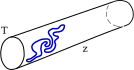
\includegraphics[width=\unitlength]{A27a-pipeSymms}}%
    \put(0.61583231,0.13683004){\color[rgb]{0,0,0}\makebox(0,0)[lb]{\smash{$z$}}}%
    \put(0.00611823,0.27217453){\color[rgb]{0,0,0}\makebox(0,0)[lb]{\smash{$\theta$}}}%
  \end{picture}%
(b)
  \begin{picture}(1,0.52454249)%
    \put(0,0){\includegraphics[width=\unitlength]{A27b-pipeSymms}}%
    \put(0.61583231,0.13683004){\color[rgb]{0,0,0}\makebox(0,0)[lb]{\smash{$z$}}}%
    \put(0.00611823,0.27217453){\color[rgb]{0,0,0}\makebox(0,0)[lb]{\smash{$\theta$}}}%
  \end{picture}%
\\
(c)
  \begin{picture}(1,0.52454249)%
    \put(0,0){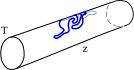
\includegraphics[width=\unitlength]{A27c-pipeSymms}}%
    \put(0.61583231,0.13683004){\color[rgb]{0,0,0}\makebox(0,0)[lb]{\smash{$z$}}}%
    \put(0.00611823,0.27217453){\color[rgb]{0,0,0}\makebox(0,0)[lb]{\smash{$\theta$}}}%
  \end{picture}%
(d)
  \begin{picture}(1,0.52454249)%
    \put(0,0){\includegraphics[width=\unitlength]{A27d-pipeSymms}}%
    \put(0.61583231,0.13683004){\color[rgb]{0,0,0}\makebox(0,0)[lb]{\smash{$z$}}}%
    \put(0.00611823,0.27217453){\color[rgb]{0,0,0}\makebox(0,0)[lb]{\smash{$\theta$}}}%
  \end{picture}%
 \end{center}
\rpo\ : recurs at
time $\period{p}$, shifted by a streamwise translation, azimuthal rotation
$g_p$
			\end{block}
%	\end{columns}
% \caption{\label{fig:A27-pipeSymms}
			\begin{exampleblock}{}
\begin{itemize}
  \item[b)]  stream-wise recurrent
  \item[c)]  stream-wise, azimuthal recurrent
  \item[d)]  azimuthal flip recurrent
\end{itemize}
			\end{exampleblock}
\end{frame}


\begin{frame}{\rpo $\to$ \po}
%%%%%%%%%%%%%%%%%%%%%%%%%%%%%%%%%%%%%%%%%%%%%%%%%%%%%%%%%%%%%%%%
%% slice.*, inflectHype.*: see dasbuch/book/FigSrc/inkscape/00ReadMe.txt
%% rpo.* hand-drawn in dasbuch/book/FigSrc/xfig/rpo.fig
%% xfig exported -> FigSrc/inkscape/rpo.fig
%% inkscape exported -> rpo.eps + LaTeX, hand edited in the macros
%% Predrag 2011-08-27 replaced rpo.pdf by rpoSlice.pdf
%%  2011-09-09 Predrag: updated continuous.tex overheads
%% remember to insert rpoSlice.pdf into ChaosBook
\begin{block}{}
 \begin{center}
  \setlength{\unitlength}{0.70\textwidth}
  %% \unitlength = units used in the Picture Environment
  \begin{picture}(1,0.87085079)%
    \put(0,0){\includegraphics[width=\unitlength]{rpoSlice}}%
    \put(0.82835153,0.19007656){\color[rgb]{0,0,0}\rotatebox{-14.84025432}{\makebox(0,0)[lb]{$\pSRed$}}}%
    \put(0.40925459,0.45713857){\color[rgb]{0,0,0}\rotatebox{0.0313674}{\makebox(0,0)[lb]{\smash{$\ssp(0)$}}}}%
    \put(0.71354118,0.39765314){\color[rgb]{0,0,0}\rotatebox{0.0313674}{\makebox(0,0)[lb]{\smash{$\sspRed(\tau)$}}}}%
    \put(0.13171187,0.38813817){\color[rgb]{0,0,0}\rotatebox{0.0313674}{\makebox(0,0)[lb]{\smash{$\LieEl(\tau)$}}}}%
    \put(0.02168739,0.31359574){\color[rgb]{0,0,0}\rotatebox{0.0313674}{\makebox(0,0)[lb]{\smash{$\ssp(\tau)$}}}}%
    \put(0.15576193,0.48769256){\color[rgb]{0,0,0}\rotatebox{0.0313674}{\makebox(0,0)[lb]{\smash{$\ssp(\period{})$}}}}%
    \put(0.54113911,0.50476963){\color[rgb]{0,0,0}\rotatebox{0.0313674}{\makebox(0,0)[lb]{\smash{$\sspRed(0)$}}}}%
  \end{picture}%
 \end{center}
\end{block}
full \statesp\ \rpo\ $\ssp(\tau)$ \\
is rotated into the \reducedsp\ {\po}
\end{frame}

\begin{frame}{relativity for pedestrians}
		\only<1>{
\begin{block}{in full \statesp}
        }
		\only<2>{
\begin{block}{in \slice}
        }
\begin{center}
		\only<1>{
(\textit{a})
  \includegraphics[width=0.40\textwidth,height=0.5\textheight,clip=true]
  {ks22rpo033p50_04p045E2}
        }
		\only<2>{
(\textit{b})
  \includegraphics[width=0.40\textwidth,height=0.5\textheight,clip=true]
  {ks22rpo033p50_04p045E2CM}
        }
\end{center}
\end{block}
		\only<1>{
a \rpo\ of the Kuramoto-Sivashinsky flow, 128$d$ \statesp\
traced for four periods
 $\period{p}$, projected on

\bigskip
full \statesp\ coordinate frame
 $\{v_1,v_2,v_3\}$; a mess
        }
		\only<2>{
a \rpo\ of the Kuramoto-Sivashinsky flow projected on

\bigskip
a slice $\{\tilde{v}_1,\tilde{v}_2,\tilde{v}_3\}$ frame
        }
\end{frame}

\begin{frame}{symmetry reduction achieved!}
\begin{itemize}
 \item all points equivalent by symmetries are represented by
    \begin{itemize}
 \item a single point
    \end{itemize}
 \item families of solutions are mapped to a single solution
    \begin{itemize}
 \item \reqva\ become \eqva
 \item \rpo s become \po s
    \end{itemize}
\end{itemize}
\end{frame}

\begin{frame}{\Large die L\"osung : \cLf\ reduced}
	\begin{columns}[t]
	\column{.50\textwidth}
 		\begin{exampleblock}{full \statesp}
        \includegraphics[width=0.7\textwidth,clip=true]
                        {CLEx1x2z} %CLEx1x2zRelEqu}
		\end{exampleblock}
	\column{.50\textwidth}
 		\begin{exampleblock}{\reducedsp}
        \includegraphics[width=0.6\textwidth,clip=true]
                        {CLEcoord245}
		\end{exampleblock}
	\end{columns}

\bigskip
ergodic trajectory was a mess, now the
topology is reveled
\\
\rpo\ \cycle{01} now a \po
\end{frame}

\begin{frame}{take-home message}
rotation into a slice \textcolor{red}{is not} an average\\
 over 3D pipe azimuthal angle

\bigskip\bigskip
it is the full snapshot of the flow embedded in the

\begin{center}
\textcolor{red}{\Large $\infty$-dimensional \statesp}
\end{center}

\bigskip\bigskip
\textcolor{red}{\Large NO information} is lost by symmetry reduction
\begin{itemize}
  \item not modeling by a few degrees of freedom
  \item no dimensional reduction
\end{itemize}
\end{frame}

\begin{frame}{slice trouble 1}
\begin{block}{portrait of \cLf\ in \reducedsp}
\begin{center}
(\textit{a})
  \includegraphics[width=0.40\textwidth,clip=true]
  {CLEcoord245}
(\textit{b})
  \includegraphics[width=0.45\textwidth,clip=true]
  {CLEperpReqb}
\end{center}
\end{block}
any choices of the slice $\slicep$
exhibit flow discontinuities
\end{frame}

\begin{frame}{slice trouble 1}
\begin{block}{glitches!}
group tangent of a generic trajectory orthogonal
to the slice tangent at a sequence of instants $\tau_k$
\[
\groupTan(\tau_k)^T \cdot \sliceTan{} = 0
\]
\end{block}
\end{frame}


\begin{frame}{Nature couples many Fourier modes}
group orbits of highly nonlinear states are highly contorted:
many extrema, multiple sections by a slice
\end{frame}

\begin{frame}{slice trouble 2}
a slice hyperplane cuts every group orbit at least twice
 \begin{columns}
 \column{0.4\textwidth}
\begin{block}{sliced wurst}
\begin{center}
%\label{fig:sliceimage}
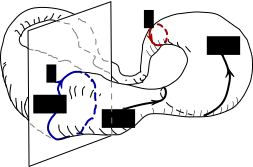
\includegraphics[width=1.00\textwidth]{A29sliceWurst}
\end{center}
\end{block}
 \column{0.6\textwidth}
      an $\SOn{2}$ \rpo\ is topologically a torus : the cuts are \po\
      images of the same \rpo, the good close one, and the rest bad ones
  \end{columns}
\end{frame}

\section{charting the \statesp}

\begin{frame}{trouble: slices cannot be global}
  \begin{columns}
  \column{0.70\textwidth}
\begin{block}{} %group orbits}
\begin{center}
  \includegraphics[width=1.00\textwidth,clip=true]
  {slicePhil}
\end{center}
\end{block}
  \column{0.30\textwidth}
representing a group orbit by the closest match
to a good template $\slicep$
(Phil Morrison)
\end{columns}
\end{frame}

\begin{frame}{trouble: slices cannot be global}
  \begin{columns}
  \column{0.70\textwidth}
\begin{block}{} %group orbits}
\begin{center}
  \includegraphics[width=1.00\textwidth,clip=true]
  {slicePhilY}
\end{center}
\end{block}
  \column{0.30\textwidth}
the `closest match'
to a bad template $\slicep$
(young Phil Morrison) can be a mismatch

\bigskip

\noindent
\textcolor{blue}{single template cannot be a good match  globally}
\end{columns}
\end{frame}

\begin{frame}{trouble: slices cannot be global}
  \begin{columns}
  \column{0.70\textwidth}
\begin{block}{} %group orbits}
\begin{center}
  \includegraphics[width=1.00\textwidth,clip=true]
  {sliceSonya}
\end{center}
\end{block}
  \column{0.30\textwidth}
representing a group orbit by the closest match
to a better template $\slicep$
(Sonya Kovalewskaya)

\bigskip

\noindent
\textcolor{blue}{to cover $\pS/\Group$ globally, need}:
\\
a set of templates:
\\\begin{itemize}
    \item 2 rolls
    \item 4 rolls
    \item ...
  \end{itemize}
\end{columns}
\end{frame}

\begin{frame}{\slice\ is good up to the {\chartBord}}
  \begin{columns}
  \column{0.46\textwidth}
%\label{fig:chartBord}  %fig:slice}
\begin{block}{}
  \setlength{\unitlength}{0.80\textwidth}
  %% \unitlength = units used in the Picture Environment
  \begin{picture}(1,0.91596465)%
    \put(0,0){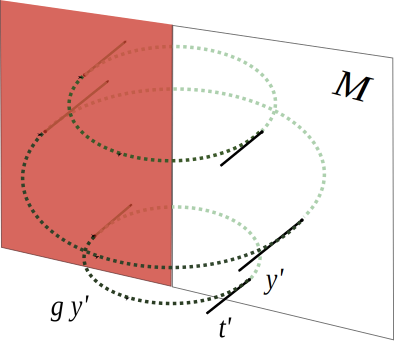
\includegraphics[width=\unitlength]{chartBord-m1}}%
    \put(0.84045332,0.67950567){\color[rgb]{0,0,0}\makebox(0,0)[lb]{\smash{$\pSRed$}}}%
    \put(0.12835189,0.11720037){\color[rgb]{0,0,0}\makebox(0,0)[lb]{\smash{$\LieEl\slicep$}}}%
    \put(0.67299795,0.18547195){\color[rgb]{0,0,0}\makebox(0,0)[lb]{\smash{$\slicep$}}}%
    \put(0.55341875,0.06171734){\color[rgb]{0,0,0}\makebox(0,0)[lb]{\smash{$\sliceTan{}$}}}%
  \end{picture}%
\end{block}
  \column{0.46\textwidth}
\begin{block}{}
  \setlength{\unitlength}{0.80\textwidth}
  \begin{picture}(1,0.91727402)%
    \put(0,0){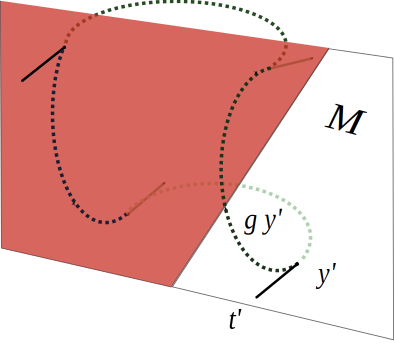
\includegraphics[width=\unitlength]{chartBord-m2}}%
    \put(0.82257887,0.59549577){\color[rgb]{0,0,0}\makebox(0,0)[lb]{\smash{$\pSRed$}}}%
    \put(0.80526889,0.1997715){\color[rgb]{0,0,0}\makebox(0,0)[lb]{\smash{$\slicep$}}}%
    \put(0.57844296,0.0831667){\color[rgb]{0,0,0}\makebox(0,0)[lb]{\smash{$\sliceTan{}$}}}%
    \put(0.61811177,0.33705605){\color[rgb]{0,0,0}\makebox(0,0)[lb]{\smash{$\LieEl\slicep$}}}%
  \end{picture}%
\end{block}
\end{columns}

$\SOn{2}$ : two hyperplanes to a given
{\template} \slicep; the slice $\pSRed$, and {\em \chartBord} $\sspRSing \in S$.
Beyond :

group orbits pierce in the wrong direction

(a) a circle group orbit  crosses the  \slice\ hyperplane twice.

(b) a group
orbit for a combination of $m=1$ and $m=2$ Fourier modes
resembles a baseball seam, and can be sliced 4 times, out of which only
the point closest to the \template\ is in the slice
\end{frame}


\begin{frame}{charting the \statesp}
for turbulent/chaotic systems a set of charts is needed to
capture the dynamics

\bigskip

\template s should be representative of the
dynamically dominant patterns seen in the solutions of nonlinear PDEs

\bigskip

we propose to construct a global atlas of the dimensionally \reducedsp\
$\pSRed$ by deploying linear \slice s $\pSRed{}^{(j)}$ across
neighborhoods of the qualitatively most important patterns $\slicep{}^{(j)}$
\end{frame}

\begin{frame}{2-chart atlas}
  \begin{columns}
  \column{0.46\textwidth}
\begin{block}{}
%\label{fig:A29-2slices}
  \setlength{\unitlength}{0.80\textwidth}
  %% \unitlength = units used in the Picture Environment
  \begin{picture}(1,0.92174023)%
    \put(0,0){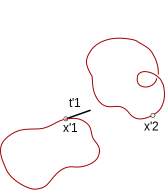
\includegraphics[width=\unitlength]{A29-2tmplts}}%
    \put(0.38186388,0.34995272){\color[rgb]{0,0,0}\makebox(0,0)[lb]{\smash{$\slicep{}^{(1)}$}}}%
    \put(0.41769945,0.50079738){\color[rgb]{0,0,0}\makebox(0,0)[lb]{\smash{$\sliceTan{}{}^{(1)}$}}}%
    \put(0.87339467,0.35886318){\color[rgb]{0,0,0}\makebox(0,0)[lb]{\smash{$\ssp'{}^{(2)}$}}}%
  \end{picture}%
\end{block}
  \column{0.46\textwidth}
\begin{block}{}
  \setlength{\unitlength}{0.80\textwidth}
  \begin{picture}(1,1.14107266)%
    \put(0,0){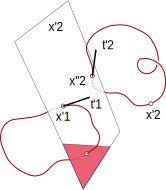
\includegraphics[width=\unitlength]{A29-2tmplSl}}%
    \put(0.54442322,0.48851386){\color[rgb]{0,0,0}\makebox(0,0)[lb]{\smash{$\sliceTan{}{}^{(1)}$}}}%
    \put(0.33649368,0.41474621){\color[rgb]{0,0,0}\makebox(0,0)[lb]{\smash{$\slicep{}^{(1)}$}}}%
    \put(0.41644523,0.62981493){\color[rgb]{0,0,0}\makebox(0,0)[lb]{\smash{$\slicep{}^{(2)}$}}}%
    \put(0.616644,0.84680609){\color[rgb]{0,0,0}\makebox(0,0)[lb]{\smash{$\sliceTan{}{}^{(2)}$}}}%
    \put(0.88017597,0.4261647){\color[rgb]{0,0,0}\makebox(0,0)[lb]{\smash{$\ssp'{}^{(2)}$}}}%
    \put(0.29194797,0.95658666){\color[rgb]{0,0,0}\makebox(0,0)[lb]{\smash{$\pSRed{}^{(1)}$}}}%
  \end{picture}%
\end{block}
\end{columns}

templates $\slicep{}^{(1)}$, $\ssp'{}^{(2)}$, with
group orbits. Start with the {\template} $\slicep{}^{(1)}$. All group
orbits traverse its $(d\!-\!1)$\dmn\ slice hyperplane, including the
group orbit of the second {\template} $\ssp'{}^{(2)}$. Replace the second
{\template} by its closest group-orbit point $\slicep{}^{(2)}$, \ie, the
point in \slice\ $\pSRed{}^{(1)}$.
\end{frame}

\begin{frame}{2-chart atlas}
  \begin{columns}
  \column{0.46\textwidth}
\begin{block}{}
%\label{fig:A29-2slices}
  \setlength{\unitlength}{1.00\textwidth}
  %% \unitlength = units used in the Picture Environment
  \begin{picture}(1,0.86567815)%
    \put(0,0){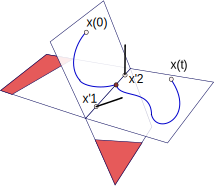
\includegraphics[width=\unitlength]{A29-2slices}}%
    \put(0.3850416,0.38725438){\color[rgb]{0,0,0}\makebox(0,0)[lb]{\smash{$\slicep{}^{(1)}$}}}%
    \put(0.60194012,0.48012421){\color[rgb]{0,0,0}\makebox(0,0)[lb]{\smash{$\slicep{}^{(2)}$}}}%
    \put(0.4042968,0.74412842){\color[rgb]{0,0,0}\makebox(0,0)[lb]{\smash{$\sspRed(0)$}}}%
    \put(0.79647438,0.54627847){\color[rgb]{0,0,0}\makebox(0,0)[lb]{\smash{$\sspRed(\zeit)$}}}%
  \end{picture}%
\end{block}
  \column{0.50\textwidth}
\begin{block}{}
  \setlength{\unitlength}{1.00\textwidth}
  \begin{picture}(1,0.5127804)%
    \put(0,0){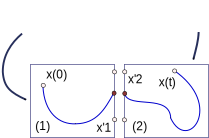
\includegraphics[width=\unitlength]{A29-2charts.pdf}}%
    \put(0.16199231,0.03841546){\color[rgb]{0,0,0}\makebox(0,0)[lb]{\smash{$\pSRed{}^{(1)}$}}}%
    \put(0.63051777,0.0374085){\color[rgb]{0,0,0}\makebox(0,0)[lb]{\smash{$\pSRed{}^{(2)}$}}}%
    \put(0.21517269,0.28787637){\color[rgb]{0,0,0}\makebox(0,0)[lb]{\smash{$\sspRed(0)$}}}%
    \put(0.75921701,0.25014044){\color[rgb]{0,0,0}\makebox(0,0)[lb]{\smash{$\sspRed(\zeit)$}}}%
    \put(0.60952792,0.26511997){\color[rgb]{0,0,0}\makebox(0,0)[lb]{\smash{$\slicep{}^{(2)}$}}}%
    \put(0.45827029,0.02997228){\color[rgb]{0,0,0}\makebox(0,0)[lb]{\smash{$\slicep{}^{(1)}$}}}%
  \end{picture}%

atlas : $(d\!-\!1)$\dmn\ charts

\end{block}
\end{columns}


2 {\template s} : the
closest points viewed from either group orbit, lie in both \slice s

\medskip

tangent vectors have different orientations : 2
\slice\ hyperplanes $\pSRed{}^{(1)}$, $\pSRed{}^{(2)}$

intersect in the \emph{ridge}, a hyperplane of dimension $(d\!-\!2)$
(here drawn as a `line')

each chart (page of the atlas above) extends only as far as this ridge

if the templates are
sufficiently close, the {\chartBord} of each \slice\ (red region) is
beyond this ridge

\end{frame}


\begin{frame}{}
\begin{center}
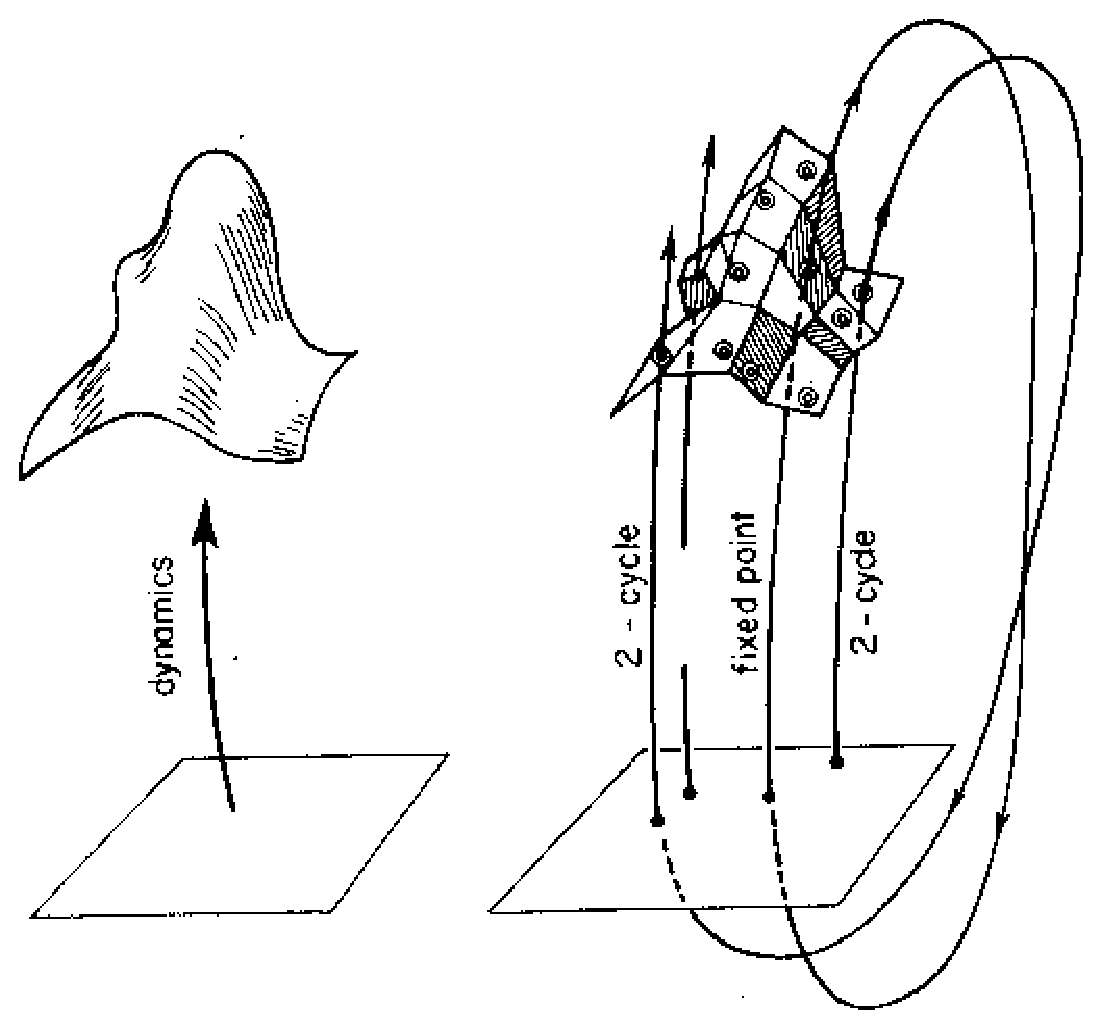
\includegraphics[width=0.60\textwidth]{f_1_08_1}
\end{center}
this is the
periodic-orbit implementation of the idea of {\statesp\ tessellation}
\end{frame}

\begin{frame}{triumph : all pipe flow solution in one happy family}
\bigskip
first 'turbulent' \rpo s for pipe flows!
\end{frame}

\section[Summary]{conclusions}

 \begin{frame}{summary}

\begin{block}{conclusion}
  \begin{itemize}
   \item 'gauge fixing' - no insight into geometry of flows
   \item symmetry reduction by \mslices:
   \\
   efficient, allows
   exploration of high-dimensional flows\\
hitherto unthinkable
  \end{itemize}
\end{block}

\begin{block}{to be done}
\begin{itemize}
  \item construct Poincar\'e sections
  \item use the information quantitatively (periodic orbit theory)
\end{itemize}
\end{block}
\end{frame}

\begin{frame}{take-home message}
if you have a symmetry
\begin{center}
\textcolor{red}{\Large use it!}
\end{center}

\bigskip\bigskip
without symmetry reduction, no understanding of fluid
flows, nonlinear field theories possible
\end{frame}

\begin{frame}{amazing theory! amazing numerics! hope...}
\begin{center}
  \includegraphics[width=0.60\textwidth,clip=true]
                    {ProblemsPill}
\end{center}
\end{frame}


\section[flotsam]{flotsam}


\end{document}
